% !TEX root = tracking.tex
\section{10D Quadrotor RRT Example \label{sec:results}}
\begin{figure*}
	\centering
	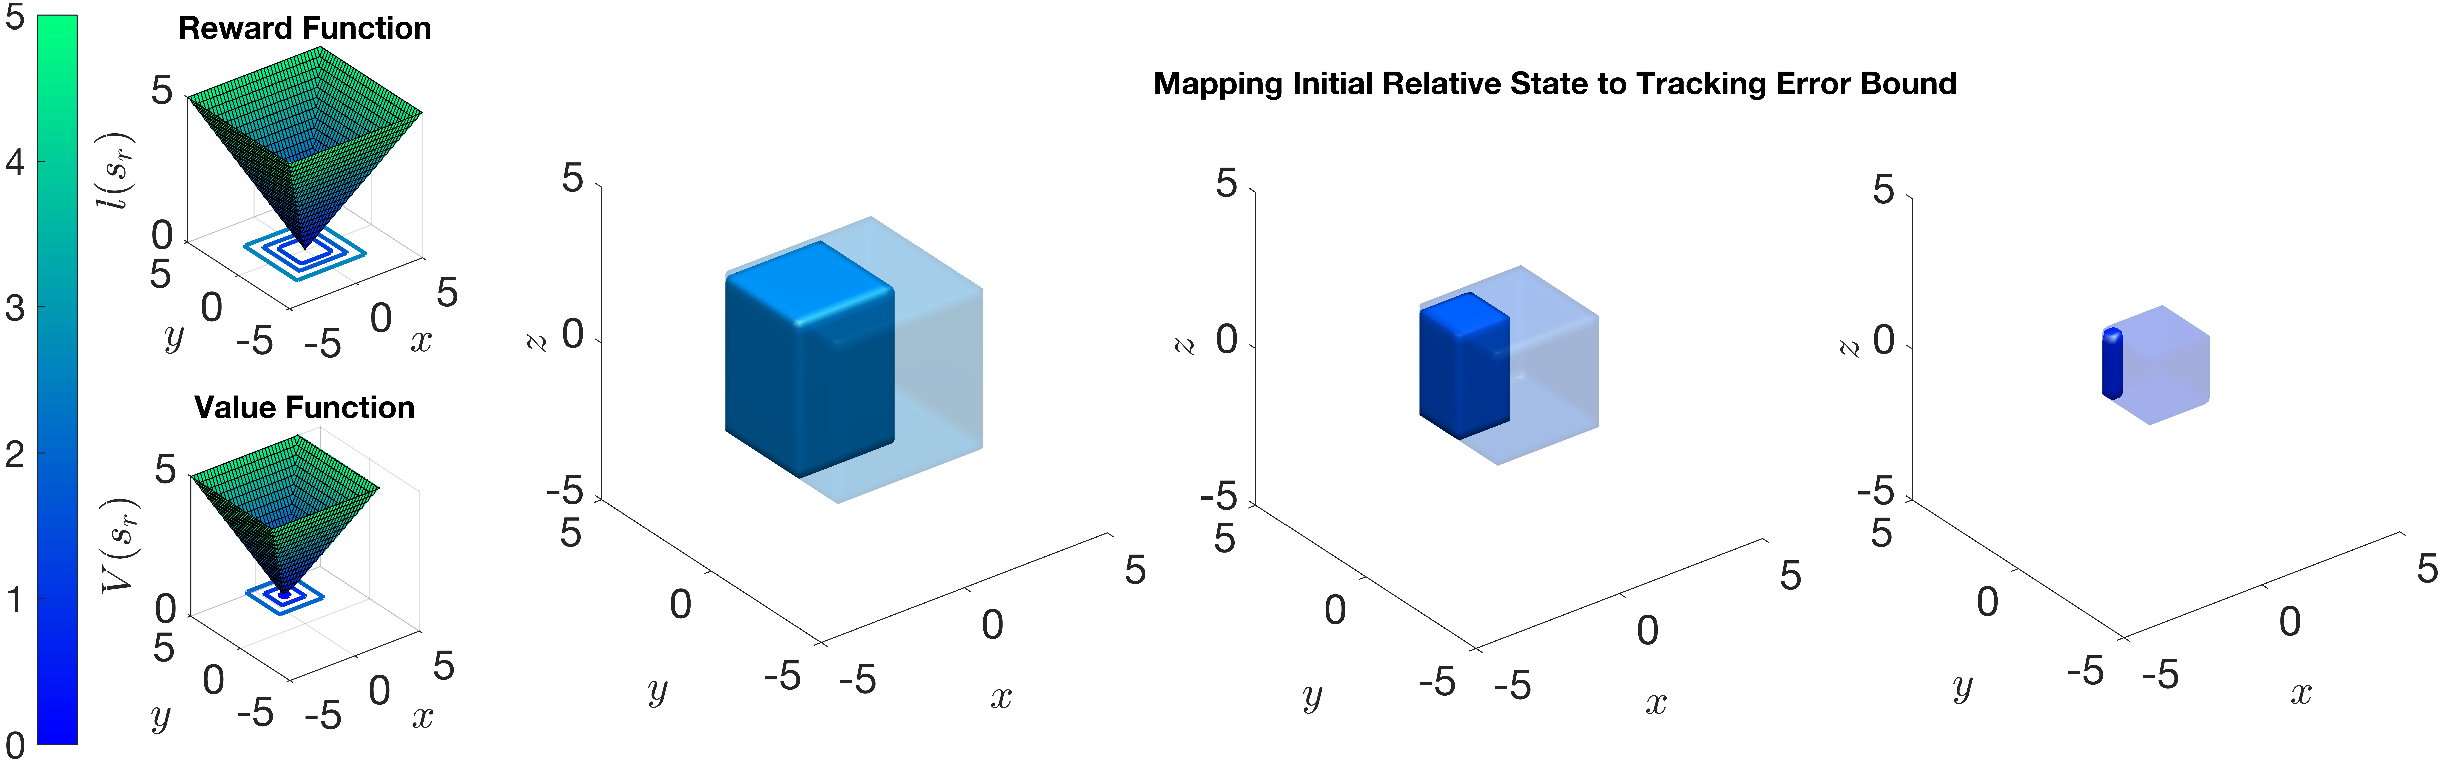
\includegraphics[width=0.9\textwidth]{fig/quad10D_example_cost}
	\caption{On the left are visualizations of the cost and value functions over a 2D slice of the 10D relative state space, with contour lines showing three level sets of these functions. The three images on the right show the 3D projections of these level sets at the same slice $(v_{xr},v_{yr},v_{zr})=[1, -1, 1]$ m/s, $(\theta_{xr},\omega_{xr},\theta_{yr},\omega_{yr})=[0,0,0,0]$. The solid boxes show the initial relative states, and the transparent boxes show the guaranteed tracking error bound around these relative states. In the online algorithm we will set the initial relative states to 0 to find the smallest invariant tracking error bound for the system.}
	\label{fig:quad10D_example}
	\end{figure*} 
\begin{figure}
	\centering
	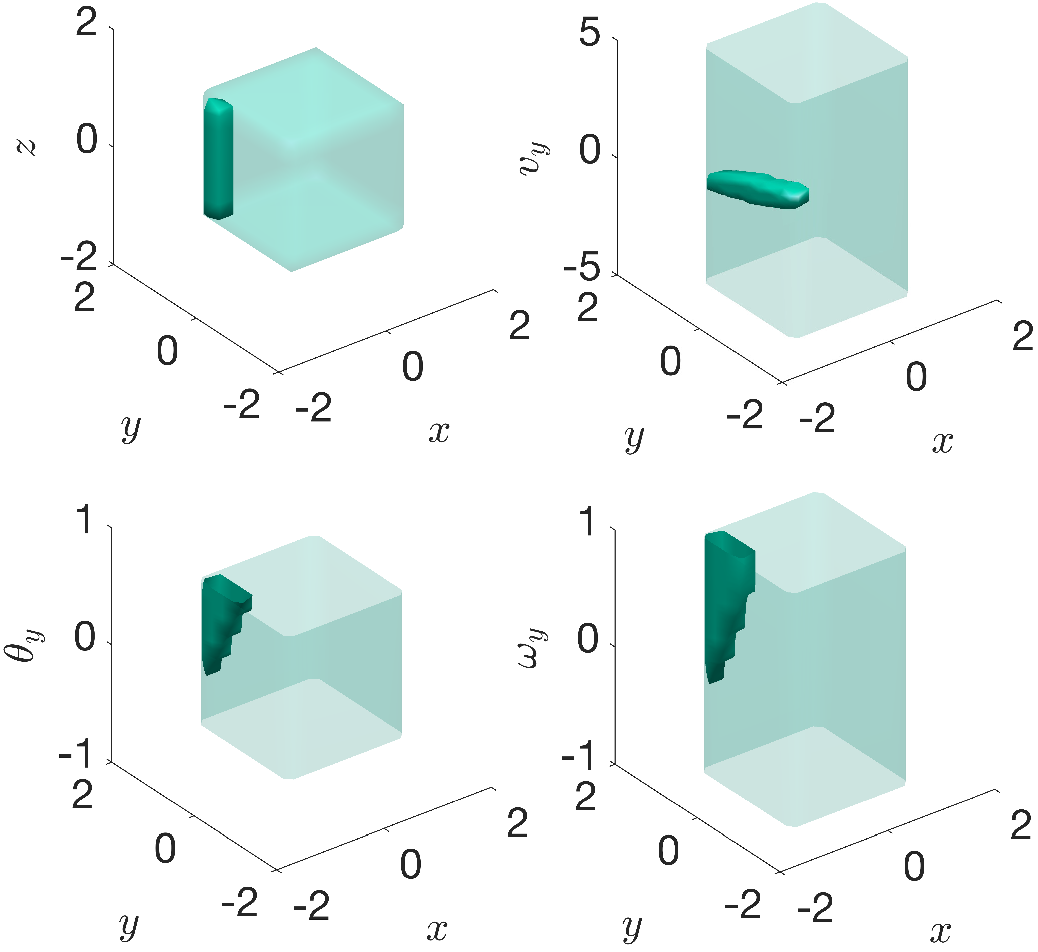
\includegraphics[width=0.3\textwidth]{fig/quad10D_slices}
	\caption{Various 3D slices along different dimensions of the 10D initial relative states (solid) and the corresponding tracking error bound (transparent)}
	\label{fig:quad10D_example_slices}
	\vspace{-.2in}
\end{figure} 
We demonstrate this framework with a 10D near-hover quadrotor developed in \cite{Bouffard12} tracking a 3D point source path generated by an RRT planner. First we perform the offline computations to acquire the tracking error bound and safety controller look-up tables. Next we set up the RRT to convert paths to simple 3D trajectories. Finally we implement the online framework to navigate the 10D system through a 3D environment with static obstacles.

\subsection{Precomputation of 10D-3D system}
First we define the 10D dynamics of the real quadrotor and the 3D dynamics of the simple point source:
\begin{equation}
\label{eq:Quad10D_dyn}
\begin{aligned}
\begin{array}{c}
\left[
\begin{array}{c}
\dot{x}\\
\dot{v_x}\\
\dot{\theta_x}\\
\dot\omega_x\\
\dot{y}\\
\dot{v_y}\\
\dot{\theta_y}\\
\dot\omega_y\\
\dot{z}\\
\dot{v_z}
\end{array}
\right]
=
\left[
\begin{array}{c}
v_x + d_x\\
g \tan \theta_x\\
-d_1 \theta_x + \omega_x\\
-d_0 \theta_x + n_0 a_x\\
v_y + d_y\\
g \tan \theta_y\\
-d_1 \theta_y + \omega_y\\
-d_0 \theta_y + n_0 a_y\\
v_z + d_z\\
k_T a_z - g
\end{array}
\right]
\left[
\begin{array}{c}
\dot{x}\\
\dot{y}\\
\dot{z}\\
\end{array}
\right]
=
\left[
\begin{array}{c}
b_x\\
b_y\\
b_z \\
\end{array}
\right]
\end{array}\\
\end{aligned}
\end{equation}
where states $(x, y, z)$ denote the position, $(v_x, v_y, v_z)$ denote the velocity, $(\theta_x, \theta_y)$ denote the pitch and roll, and $(\omega_x, \omega_y)$ denote the pitch and roll rates. The controls of the 10D system are $(a_x, a_y, a_z)$, where $a_x$ and $a_y$ represent the desired pitch and roll angle, and $a_z$ represents the vertical thrust. The 3D system controls are $(b_x, b_y, b_z)$, and represent the velocity in each positional dimension. The disturbances in the 10D system $(d_x, d_y, d_z)$ are caused by wind, which acts on the velocity in each dimension. Next the relative dynamics between the two systems is defined using (\ref{eq:rdyn}):
\begin{equation}
\label{eq:Quad10DRel_dyn}
\begin{aligned}
\begin{array}{c}
\left[
\begin{array}{c}
\dot{x_r}\\
\dot{v_{xr}}\\
\dot{\theta_{xr}}\\
\dot\omega_{xr}\\
\dot{y_r}\\
\dot{v_{yr}}\\
\dot{\theta_{yr}}\\
\dot\omega_{yr}\\
\dot{z_r}\\
\dot{v_{zr}}
\end{array}
\right]
=
\left[
\begin{array}{c}
v_x - b_x + d_x\\
g \tan \theta_x\\
-d_1 \theta_x + \omega_x\\
-d_0 \theta_x + n_0 a_x\\
v_y - b_y + d_y\\
g \tan \theta_y\\
-d_1 \theta_y + \omega_y\\
-d_0 \theta_y + n_0 a_y\\
v_z - b_z + d_z\\
k_T a_z - g
\end{array}
\right]
\end{array}\\
\end{aligned}
\end{equation}
The values for parameters $d_0,d_1,n_0,k_T,g$ used were: $d_0=10,d_1=8,n_0=10,k_T=0.91,g=9.81$. The 10D control bounds were $|a_x|,|a_y|\leq10$ degrees, $0\leq a_z\leq 1.5g$ m/s$^{2}$. The 3D control bounds were $|b_x|,|b_y|,|b_z|\leq0.5$ m/s. The disturbance bounds were $|d_x|,|d_y|,|d_z|\leq0.1$ m/s.

Next we follow the setup described in section \ref{sec:precomp} to create a cost function, which we then evaluate using HJ reachability until convergence to produce the invariant value function as in (\ref{eq:valfunc}). Historically this 10D nonlinear relative system would be intractable for HJ reachability analysis, but using new methods in \cite{Chen2016b} we can decompose this system into 3 subsystems (one for each positional dimension). To do this we must also decompose the cost function, resulting in a one-norm instead of a two-norm. This cost function as well as the resulting value function can be seen projected onto the $x,y$ dimensions in Figure \ref{fig:quad10D_example}.

Figure \ref{fig:quad10D_example} also shows 3D positional projections of the mapping between initial relative state to maximum potential relative distance over all time (i.e. tracking error bound). If the real system starts exactly at the origin in relative coordinates, its tracking error bound will be a box of 0.81 meters in each direction. Slices of the 3D set and corresponding tracking error bounds are also shown in \ref{fig:quad10D_example_slices}. We save the look-up tables of the value function (i.e. the tracking error function) and its spatial gradients (i.e. the safety controller function).

\subsection{RRT Online Planning}
\textcolor{red}{what RRT planner we're using, how we convert it to dynamics, setup of environment, results}

\textcolor{cyan}{SooJean's words: How obstacles are sensed, how obstacles are expanded to account for the tracking error bound. Three types of obstacles: all, local, expanded. How my part fits into the overall model: take in a point (may account for disturbance in the model) and compute the entire RRT path (this step is the "online") from there. Local and expanded obstacles are updated along the way.}